\section{Samlet kredsløb} \label{bilag:samletkreds}
\begin{figure}[H]
  \centering
  \caption{Et billede af det samlede kredsløb}
  \label{}
\end{figure}
\newpage


\section{PCB artwork til hastighedssensor}\label{bilag:afsenderModtagerArtwork}
\begin{figure}[H]
	\centering
    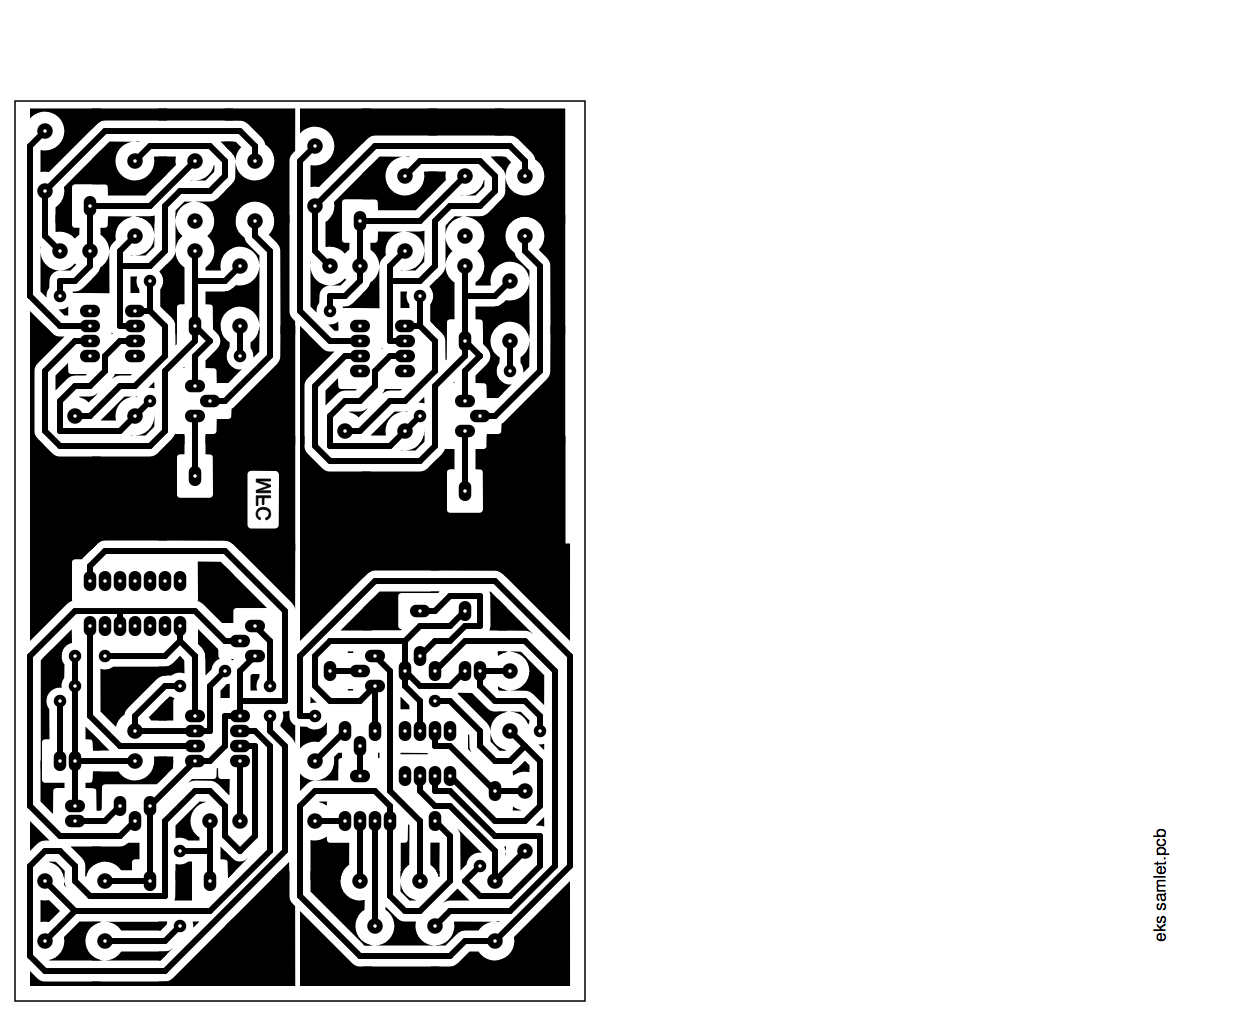
\includegraphics[width=210mm]{figures/2_5fremstilling/afsenderModtagerArtwork.png}
\end{figure}


\section{PCB artwork til arduino shield} \label{bilag:shieldArtwork}
\begin{figure}[H]
	\centering
    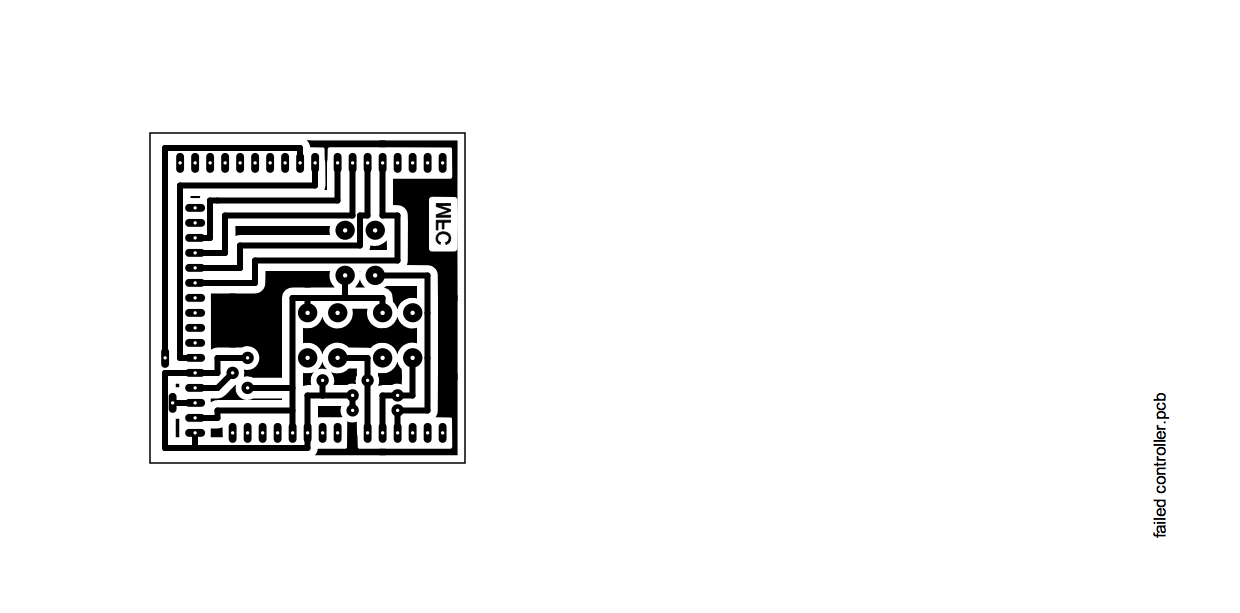
\includegraphics[width=210mm]{figures/2_5fremstilling/shieldArtwork.png}
\end{figure}

\todo{Måske skulle vi overveje at lave et nyt billede med samlede kabler}
\begin{figure}[H]
\section{Fumlebrætmodel anden del}
	\centering
    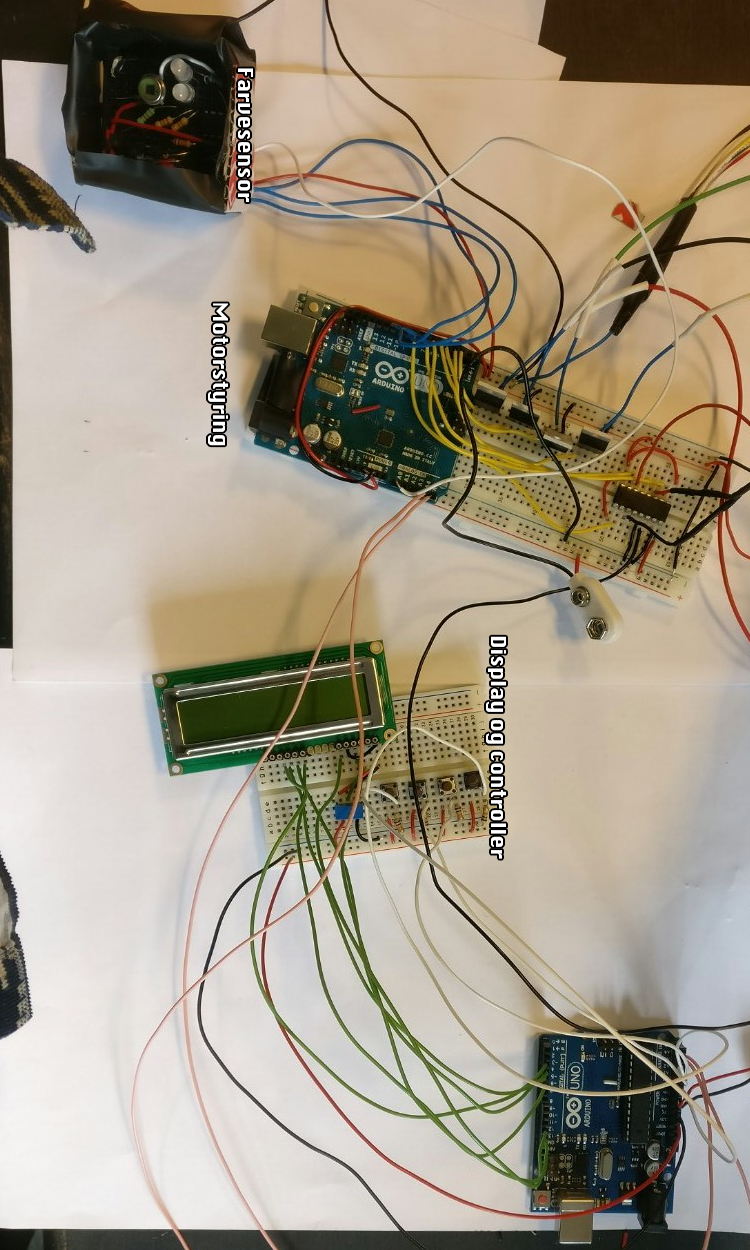
\includegraphics[width=13cm]{figures/2_5fremstilling/prototyper/rumleKreds.png}
\end{figure}

% Must be second last (the longer the later)
\section{Program til Arduino}
\label{bilag:program}
\begin{lstlisting}

\end{lstlisting}


% MUST BE LAST
\section{Logbog} 